\documentclass{article}
\usepackage{neurips_2026}
\usepackage[utf8]{inputenc}
\usepackage[T1]{fontenc}
\usepackage{hyperref}
\usepackage{url}
\usepackage{booktabs}
\usepackage{amsfonts,amsmath}
\usepackage{nicefrac}
\usepackage{microtype}
\usepackage{xcolor}
\usepackage{graphicx}
\graphicspath{{../figures/}}

\title{How Fragile Are Pairwise-Comparison Leaderboards? \\
Worst-Case and Benign Perturbations of Bradley--Terry Rankings Across Evaluation Designs}

\author{Anonymous Authors}

\begin{document}
\maketitle

\begin{abstract}
Pairwise-comparison leaderboards such as Chatbot Arena rank participants by a Bradley--Terry (BT) fit to many ``A versus B'' outcomes and are used for model selection and marketing, yet it is unclear how much the displayed ranking depends on individual comparisons.
We measure this with \emph{verified worst-case perturbations}: an influence-function search for the smallest set of comparisons to remove, flip or inject so that a ranking decision changes, with every reported budget confirmed by an exact refit, and compare it with benign noise (bootstrap, random removal or flipping).
On four real datasets from three evaluation designs (Arena crowd votes, MT-Bench expert and GPT-4 verdicts, NBA games), the point ranking is often extremely fragile: changing the top-1 requires altering 1--2 of 57\,477 Arena comparisons and about 9 of 59\,008 NBA games, but 46--166 of 2\,400--3\,355 MT-Bench verdicts.
The budget tracks the target's gap in standard errors (Spearman correlation 0.86--0.96 on the 63 Arena and 44 NBA adjacent pairs) and, in labelled synthetic calibration, scales like $z\sqrt{N/p}$.
For Arena and NBA these swaps lie within sampling noise: bootstrap resampling alone changes the Arena top-1 in about half of the resamples, and the cheapest point-rank top-1 attack leaves the confidence-interval-based published rank of Arena and NBA unchanged (we did not search for attacks aimed at the published rank).
Differences between datasets are confounded with size, number of participants and gap structure; at matched size and participant count the spread of top-1 budgets shrinks from about 80-fold to about 7-fold, and GPT-4 verdicts on the same questions are more stable than expert votes.
Our budgets are upper bounds on the true minimum, and our conclusions concern fixed snapshots and BT fits.
\end{abstract}

\section{Introduction}\label{sec:intro}
Leaderboards built from pairwise comparisons---Chatbot Arena being the prominent example \citep{chiang2024arena}---fit a Bradley--Terry (BT) model \citep{bradley1952} to many ``A versus B'' outcomes and publish the ranking, often with confidence intervals. Practitioners use such rankings to pick models, and providers cite them in announcements. How much a ranking depends on individual comparisons is therefore a practical question, whether the change comes from noise or from deliberate action \citep{min2025rigging,singh2025illusion}.

We ask: \emph{what is the smallest change to the comparison data that changes a decision a reader takes from the leaderboard, how does this compare with benign noise, and does it differ across datasets and evaluation designs?}
We make this operational by (i) fixing decisions (rank~1, the order of adjacent pairs, top-$k$ sets, Kendall's $\tau$, and the published rank derived from confidence intervals), (ii) searching for the smallest verified removal, flip or injection that changes each decision, (iii) comparing with bootstrap and random perturbation, and (iv) comparing datasets on a common footing using the standardised gap and size/participant controls instead of raw counts.

\paragraph{Contributions.}
(1) A verified-budget methodology for rank decisions of BT leaderboards that adapts influence-function robustness analysis \citep{koh2017influence,broderick2020amip} and reports approximation errors.
(2) Measurements on four real datasets from three evaluation designs with bootstrap spread: point-rank decisions can flip with a handful of comparisons where gaps are small, but on Arena and NBA these flips are within sampling noise, and the cheapest point-rank attack does not change a confidence-interval-based rank (attacks aimed at that rank were not searched).
(3) A scale that explains the differences: the budget follows the gap in standard errors, and in labelled synthetic worlds scales like $z\sqrt{N/p}$, so cross-dataset differences track size, participants and gap structure and cannot be attributed to the evaluation design with these data.
(4) Explicit scope: our budgets are upper bounds, from fixed snapshots, with optimistic bootstrap intervals.

\section{Related Work}\label{sec:related}
\paragraph{Pairwise-comparison leaderboards.}
The Bradley--Terry (BT) model \citep{bradley1952} underlies the rankings of Chatbot Arena, which
aggregates crowd votes between anonymous model pairs and reports BT scores with confidence
intervals \citep{chiang2024arena}. MT-Bench releases expert and GPT-4 pairwise judgments
\citep{zheng2023judge}, a second, differently produced comparison design.
BT estimation has many extensions, among them ties and covariates such as a home-advantage term \citep{hunter2004mm,turner2012bt2}, which we use for sports data.
\paragraph{Critiques and manipulation of Arena.}
\citet{min2025rigging} study vote-rigging strategies that raise a model's rank, and
\citet{singh2025illusion} document data-access and sampling asymmetries in Arena's practice.
Both concern \emph{how} the comparison data can be altered or are non-uniformly collected; we ask how much
alteration a fixed snapshot tolerates, under removals, flips and injections, and compare this with benign noise
and across designs.
\paragraph{Robustness to dropping data.}
Influence functions \citep{koh2017influence} give first-order effects of single observations, and
\citet{broderick2020amip} turn them into a search for the small subset whose removal most changes an analysis conclusion,
verified by refitting. We adapt this approach to ranking decisions of a BT fit.

\section{Method}\label{sec:method}
\paragraph{Leaderboard.}
A dataset is a list of $N$ comparisons $c=(i_c,j_c,y_c)$ between participants $i_c,j_c\in\{1,\dots,p\}$ with outcome $y_c\in\{0,\tfrac12,1\}$ (score of $i_c$; $\tfrac12$ is a tie).
The leaderboard is the Bradley--Terry (BT) fit \citep{bradley1952}: $P(i\text{ beats }j)=\sigma(\theta_i-\theta_j)$, and
$\hat\theta$ minimises the logistic loss $-\sum_c [\,y_c\log\sigma(\eta_c)+(1-y_c)\log(1-\sigma(\eta_c))\,]+\tfrac{\lambda}{2}\|\theta\|^2$,
$\eta_c=\theta_{i_c}-\theta_{j_c}$, with a weak ridge $\lambda=10^{-3}$ that fixes the additive gauge and keeps the fit finite under perfect separation.
Ties count as half a win to each side. For sports data an additional shared home-advantage term enters $\eta_c$.
The ranking is $\mathrm{argsort}(-\hat\theta)$; scores are in natural log-odds units.
Bootstrap confidence intervals resample the $N$ comparisons with replacement.
\paragraph{Decisions.}
We do not perturb scores but the \emph{decisions} a reader takes from a leaderboard:
(a) the identity of rank~1; (b) the order of an adjacent pair; (c) the top-$k$ set (Appendix Table~\ref{tab:topk}); (d) Kendall's $\tau$ against the original ranking falling below 0.95 or 0.9;
(e) the \emph{published-style} rank $1+\#\{j:\mathrm{lo}_j>\mathrm{hi}_i\}$ computed from 95\% score intervals, which is what a leaderboard with confidence intervals displays.
Targets (the top pair, and every adjacent pair of the original ranking) are fixed by the original ranking before any attack is run.
\paragraph{Perturbation models and budget.}
We consider three alterations of the comparison data: \emph{drop} $m$ comparisons, \emph{flip} the outcome of $m$ comparisons, and \emph{inject} $m$ new comparisons that involve the target (win for the promoted participant against some opponent, or loss of the leader).
The budget is $m$, also reported as $m/N$ and relative to the number of comparisons carried by the target participants.
\paragraph{Worst-case search.}
For a target pair $(a,b)$ with $a$ ranked above $b$ we look for a small set of alterations after which $\hat\theta_a\le\hat\theta_b$.
Per comparison, the first-order effect on $\hat\theta_a-\hat\theta_b$ is given by the influence function of the penalised BT likelihood \citep{koh2017influence},
the same approximation that \citet{broderick2020amip} use to find the small data subset whose removal changes a conclusion.
We rank comparisons by this effect, alter the best batch, refit exactly, and repeat; then we bisect over the prefix of the alteration order, so the reported budget $m^\star$ is always verified by an exact refit of the altered data.
For injection, all $m$ new votes involve the target and a single opponent, chosen among the six most promising by the first-order screen and verified by exact refits. Attacks that succeed only by disconnecting the comparison graph are discarded.
Because the search is greedy, $m^\star$ is an \emph{upper bound on the minimum} number of alterations: a found attack proves that the decision is that fragile, while the absence of an attack proves nothing about robustness; we have no certified lower bound.
For Kendall's $\tau$ we apply the cheapest adjacent-swap attack repeatedly until $\tau$ drops below the threshold.
Baselines restrict the alterations to head-to-head comparisons of the target pair, or to comparisons involving either target.
\paragraph{Benign noise and scale.}
As benign perturbations we use bootstrap resampling, random dropping and random flipping of $m$ comparisons; we report the probability that each decision changes (Wilson intervals).
To compare datasets of different size we express the scale of a decision in two ways: the gap of the targeted pair in bootstrap standard-error units, and the subsample fraction $b_q$ of $N$ at which the decision flips with probability $q$ under random subsampling (reported with censoring flags when outside the grid).

\section{Experimental Setup}\label{sec:setup}
\paragraph{Data.}
We use four real comparison sets from three evaluation designs, all public snapshots pinned by commit and checksum (Appendix~\ref{app:repro}).
\emph{Crowd votes:} Chatbot Arena human preference data (57\,477 battles between 64 models; HF \texttt{lmarena-ai/arena-human-preference-55k}, apache-2.0). Ties and ``both bad'' are merged into ties.
\emph{Expert and model-judge verdicts:} MT-Bench human judgments (3\,355 votes on 6 models) and GPT-4 pairwise judgments of the same models (2\,400 verdicts; ``inconsistent'' verdicts are treated as ties) \citep{zheng2023judge}; 1\,814 questions are covered by both.
\emph{Sports:} the FiveThirtyEight NBA game file, one row per game after removing the duplicate \texttt{\_iscopy} rows, NBA league only (the 1968--76 ABA is a separate, weakly connected league and is analysed as its own leaderboard where mentioned), 59\,008 games between 45 franchises when pooled over all seasons and 78 single regular seasons analysed separately; the BT model has one shared home-advantage parameter.
We did not use the optional larger Arena set, WebDev Arena, or the LLM-judge verdicts on Arena battles (deferred in the study plan for budget reasons).
\paragraph{Targets, seeds and repeats.}
Targets are fixed from the original ranking before attacks run: the top-1 pair, every adjacent pair, and Kendall's $\tau$ thresholds.
Bootstrap resamples (with replacement over comparisons) quantify the sampling spread of each adversarial budget; random-perturbation baselines use Monte-Carlo draws; all seeds are fixed in the scripts (Appendix~\ref{app:repro}).
Arena rows have no user identifier and repeat prompts (51\,734 distinct prompts in 57\,477 rows), so treating comparisons as independent makes bootstrap intervals optimistic.
\paragraph{Controls for size and design.}
Datasets differ in size, number of participants, tie rate and structure, so cross-dataset differences are not attributed to ``design''.
Clean contrasts are (i) MT-Bench expert versus GPT-4 verdicts on the same questions, (ii) Arena subsampled to the size of MT-Bench (all 64 models) and restricted to its six strongest models, and (iii) variation across NBA seasons.
\paragraph{Prior work on this question.} The task statement noted that its question has been studied in a published paper that must not be consulted. One starter-list entry appeared to match that description, so we did not read, cite or search for it; no forbidden material was encountered (see \texttt{REPRODUCE.md}).
\paragraph{Compute and LLM assistance.}
All experiments run on CPU (2 cores). LLM assistance (Claude Sonnet 5.5, via Claude Code) was used for literature reading, code, analysis and writing of this paper and all numbers, figures and tables are produced by the shipped code.

\section{Results}\label{sec:results}
All budgets are the smallest verified attacks we found (upper bounds on the minimum). ``Remove'', ``flip'' and ``inject'' are the three alteration types; $N$ is the number of comparisons.

\paragraph{Point rankings can flip with a handful of comparisons.}
Table~\ref{tab:summary} gives the smallest attack changing the top-1 and pushing Kendall's $\tau$ below 0.95. On Arena-55k (57\,477 battles, 64 models) the top-1 changes after removing 2 comparisons, flipping 1, or injecting 2 (0.003\% of $N$); in the pooled NBA data (59\,008 games) after removing 9 or flipping 6. On MT-Bench the same decision needs 92 removals or 46 flips with expert votes ($N=3355$) and 166 or 61 with GPT-4 verdicts ($N=2400$), i.e.\ 1.4--6.9\% of $N$. The ranking as a whole is less brittle than its leader: for $\tau<0.95$ the smallest attacks remove 56 comparisons on Arena (0.10\%), 21 on NBA (0.04\%), 13 on MT-Bench expert (0.39\%) and 82 on GPT-4 (3.4\%).
In one of six resamples the Arena $\tau<0.9$ flip attack found no attack within 50\% of $N$ (the budget there is censored); for pair decisions the subsample fraction $b_{50}$ is not reached, so we report $b_{10}$ and $b_{25}$ with grid flags in \texttt{results/summary\_b50.csv}. Over all adjacent pairs of the original ranking, 95\% of the Arena pairs and 95\% of the NBA pairs have a gap below two standard errors, 63\% and 70\% respectively can be swapped by at most ten removals, and the median swap needs 5 (Arena) or 5.5 (NBA) removals. The smallest swap budget rises with the gap $z$ (Figure~\ref{fig:gap}, Appendix Table~\ref{tab:gapfit}; Spearman correlation between budget and $z$: 0.96 and 0.95 on Arena (63 pairs; removal, flip), 0.87 and 0.86 on NBA (44 pairs), 0.97--1.0 on the five MT-Bench pairs). Over 78 single NBA regular seasons the top-1 changes after a median of 4 removals (95\% bootstrap interval of the median 3--5; 0.56\% of the season's games) at a median leader gap of 0.64 standard errors. Of the 78 season leaderboards, 12 have an exact tie between the top two teams (budget 0). The first-order influence estimate matches the exact-refit budget on Arena and NBA (median ratio 1.0) but is off by a factor 0.94--1.97 on MT-Bench, where budgets are large; the reported budgets are always the verified ones.

\paragraph{On Arena and NBA these changes are within sampling noise.}
Bootstrap resampling of all comparisons changes the Arena top-1 in 48\% of 100 resamples (Wilson 95\% interval 38--58\%) and the NBA top-1 in 37\% (28--47\%), but never in 200 benign bootstrap resamples of either MT-Bench source (where the budgets are large) (one-sided 95\% bound 1.9\%). Random removal or flipping of as many comparisons as the cheapest attack changes the top-1 only rarely (Table~\ref{tab:benign}, Figure~\ref{fig:benign}): for example 0 of 200 random removals of 2 comparisons and 4 of 200 random flips of 10 on Arena. Sampling-scale noise is not negligible: even when random subsamples keep 90\% of the data the Arena top-1 differs from the full-data leader in 46\% of 100 draws, and in 24\% for NBA (\texttt{results/subsample\_*.csv}). Random flips do move the Arena top-1 once they reach roughly $0.1$--$1\%$ of $N$ (Figure~\ref{fig:benign}b). So the worst case needs far fewer alterations than random noise of the same size would use to move the ranking, but it exploits a gap that sampling already leaves open. The published-style rank, which accounts for confidence intervals, is unaffected: after the cheapest top-1 attack on Arena or NBA no model changes its published rank, although two models change their point rank; on MT-Bench one or two models change their published rank at the larger budgets (Table~\ref{tab:pubrank}).

\paragraph{Design versus size.}
Across datasets the top-1 budget differs by about 80-fold in comparison counts (2 on Arena, 166 on MT-Bench GPT-4; Table~\ref{tab:summary}), but datasets differ in size, number of participants, tie rate and gap structure at once. Figure~\ref{fig:design}(b) separates some factors. Subsampling Arena to the size of MT-Bench ($N=2400$ or $3355$, all 64 models) leaves the top-1 budget at 1--2 removals (median over 50 subsamples), as on the full data, so size alone does not explain the MT-Bench robustness. Restricting Arena to its six highest-ranked models, which are near-tied GPT-4 variants, raises it to a median of 11.5 removals on 2\,400 comparisons (14 on all 3\,222); this control is not comparable with the random-six control below. In the control with $N=2000$ comparisons and six participants (six random models or teams among the 20 most compared; for MT-Bench the six fixed models), the median top-1 removal budget is 60 on Arena, 20.5 on NBA, 56 on MT-Bench expert and 138.5 on MT-Bench GPT-4. The spread is then about 7-fold instead of 80-fold, with the GPT-4 verdicts the most stable. With $N=2000$ and all participants the median budget is 2 on Arena (the graph was connected in 99 of 100 subsamples) and 55 and 140.5 on MT-Bench; the same control on NBA disconnects the graph in most subsamples and is not used. On the same 1\,814 questions (Figure~\ref{fig:design}(a)), the removal budget for the top-1 is 103.5 (bootstrap interval of the median 96--110) for GPT-4 verdicts, but 41 (39--43) for one randomly chosen expert vote per question; the standardised top-1 gap on the original data is 5.5 for GPT-4 and 4.1 for all expert votes. This is a contrast of two judges on the same items, not of ``experts versus crowds''.

\paragraph{Modelling choices.}
The Arena leader is itself sensitive to the tie rule: with ties dropped (39\,716 battles) the leader changes from gpt-4-1106-preview to gpt-4-0125-preview, with the top-1 removal budget rising from 2 to 9 (Appendix Table~\ref{tab:sens}). Ridge strength (from $10^{-5}$ to $10^{-1}$) and, for NBA, the home term change the ranking little (Kendall $\tau\ge0.976$ with the primary fit) and leave the top-1 budgets within 1 comparison.

\paragraph{What predicts fragility.}
In simulated BT worlds (\textbf{synthetic}; calibration only) the log top-1 removal budget regresses on $\log z$ (coefficient 0.91, 95\% interval 0.85--0.96), $\log N$ (0.49) and $\log p$ ($-0.49$) with $R^2=0.98$, i.e.\ the budget scales roughly like $z\sqrt{N/p}$ (Appendix Figure~\ref{fig:synth}). For the cheapest adjacent swap the fitted coefficient on $\log p$ is $-1.93$ (95\% interval $-2.12$ to $-1.76$) and on $\log z$ 0.08 (\texttt{results/summary\_synthetic\_regression.csv}): with many participants some pair is nearly tied, so the first swap is cheap.

\begin{table}[t]\caption{Smallest verified attack found, in percent of $N$ (bootstrap 2.5--97.5 percentiles in brackets, from 20 resamples for the Arena and NBA top-1 rows and 100 for MT-Bench; the Arena and NBA $\tau$ rows have only 6 resamples and show the point value). Top-1: the decision changes; $\tau$: Kendall's $\tau$ against the original ranking falls below 0.95.}\label{tab:summary}\centering
{\footnotesize\setlength{\tabcolsep}{3pt}\begin{tabular}{@{}lrrccc@{}}\toprule
Dataset & $N$ & $p$ & remove & flip & inject\\\midrule
\multicolumn{6}{@{}l}{\emph{top-1 changes}}\\
Arena 55k & 57\,477 & 64 & 0.003 [0.003, 0.091] & 0.002 [0.002, 0.059] & 0.003 [0.003, 0.12] \\
MT-Bench expert & 3\,355 & 6 & 2.74 [1.58, 4.13] & 1.37 [0.80, 1.97] & 2.71 [1.58, 3.92] \\
MT-Bench GPT-4 & 2\,400 & 6 & 6.92 [4.25, 8.86] & 2.54 [2.02, 2.96] & 5.04 [4.02, 5.92] \\
NBA & 59\,008 & 45 & 0.015 [0.002, 0.070] & 0.010 [0.002, 0.045] & 0.019 [0.003, 0.088] \\
\midrule
\multicolumn{6}{@{}l}{\emph{Kendall $\tau<0.95$}}\\
Arena 55k & 57\,477 & 64 & 0.097 & 0.061 & -- \\
MT-Bench expert & 3\,355 & 6 & 0.39 [0.030, 1.54] & 0.21 [0.030, 0.77] & -- \\
MT-Bench GPT-4 & 2\,400 & 6 & 3.42 [2.23, 4.25] & 1.62 [1.12, 1.96] & -- \\
NBA & 59\,008 & 45 & 0.036 & 0.063 & -- \\
\bottomrule\end{tabular}}
\end{table}
\begin{figure}[t]\centering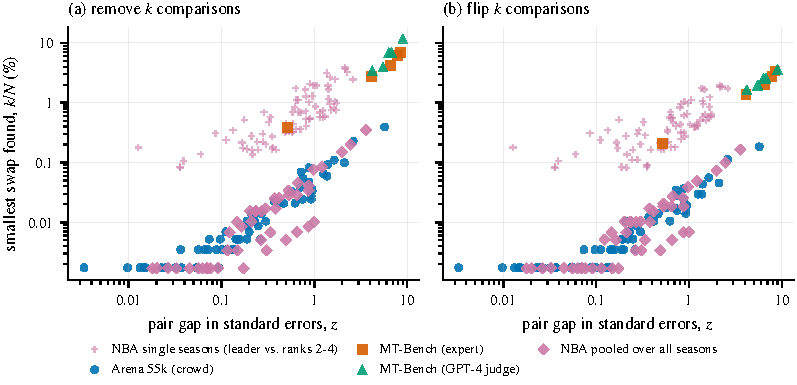
\includegraphics[width=\linewidth]{fig1_fragility_vs_gap.pdf}\caption{Smallest verified swap of an adjacent pair, as a fraction of $N$, against the pair's gap in standard errors; (a) removals, (b) flips; log-log axes. Markers: adjacent pairs of the full-data ranking of each dataset (NBA pooled over all seasons); crosses: NBA single seasons (leader against ranks 2--4). Many Arena pairs sit at the floor of one comparison. Upper bounds on the minimum.}\label{fig:gap}\end{figure}
\begin{figure}[t]\centering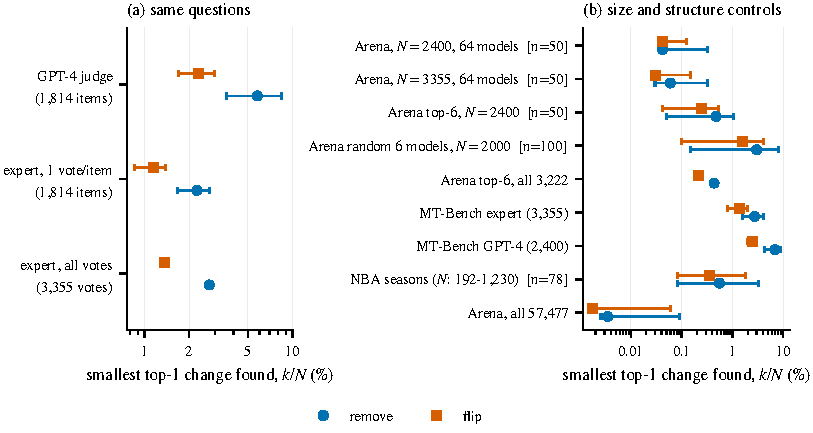
\includegraphics[width=\linewidth]{fig2_design_control.pdf}\caption{Top-1 budget. (a) The same 1\,814 MT-Bench questions judged by experts and by GPT-4. (b) Size and structure controls fixed before running; rows marked $[n{=}\cdot]$ show the median over $n$ subsamples with 2.5--97.5 percentile bars; full-data rows show the original-data value with a 2.5--97.5 percentile bootstrap bar where resamples exist; ``1 vote/item'' is the median over 100 random one-vote-per-question draws. The top-6 rows (the six highest-ranked models, near-tied GPT-4 variants) are not comparable with the random-six-models row. Cross-dataset differences are confounded with $N$, number of participants, ties and structure.}\label{fig:design}\end{figure}
\begin{figure}[t]\centering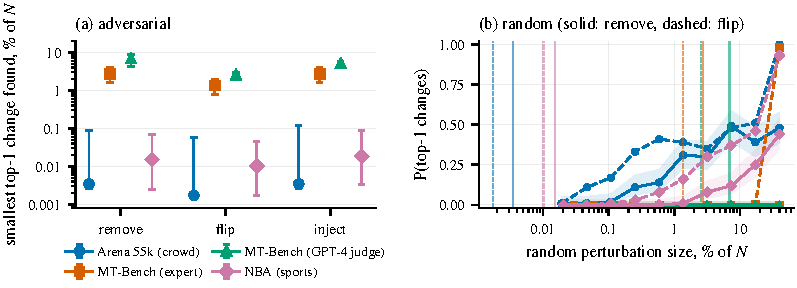
\includegraphics[width=\linewidth]{fig3_top1_adv_vs_benign.pdf}\caption{(a) Smallest verified top-1 attack by removing, label-flipping or injecting votes: dot, original data; bar, 2.5--97.5 percentile over bootstrap resamples (drawn for at least 20 resamples; Arena and NBA have 20). (b) Probability that random removal (solid) or flipping (dashed) of $m$ comparisons changes the top-1, colours as in (a); Wilson 95\% band for removal only; vertical lines mark the adversarial budgets.}\label{fig:benign}\end{figure}
\begin{table}[t]\caption{Effect of the cheapest top-1 attack (removal or flip, $k$ comparisons) on the published-style rank (95\% Wald intervals): the new point-rank leader, the number of models at published rank 1 before $\to$ after, and the number of models whose point rank ($\Delta$ point) or published rank ($\Delta$ pub.) changes. Published rank 1 is shared when intervals overlap.}\label{tab:pubrank}\centering
{\scriptsize\setlength{\tabcolsep}{3pt}\begin{tabular}{@{}llrlccc@{}}\toprule
Dataset & attack & $k$ & new leader & \# at pub.\ rank 1 & $\Delta$ point ranks & $\Delta$ pub.\ ranks\\\midrule
Arena 55k & drop & 2 & gpt-4-0125-preview & 2 $\to$ 2 & 2 & 0 \\
Arena 55k & flip & 1 & gpt-4-0125-preview & 2 $\to$ 2 & 2 & 0 \\
MT-Bench expert & drop & 92 & claude-v1 & 1 $\to$ 2 & 2 & 2 \\
MT-Bench expert & flip & 46 & claude-v1 & 1 $\to$ 2 & 2 & 2 \\
MT-Bench GPT-4 & drop & 166 & claude-v1 & 1 $\to$ 2 & 2 & 1 \\
MT-Bench GPT-4 & flip & 61 & claude-v1 & 1 $\to$ 2 & 2 & 1 \\
NBA & drop & 9 & Lakers & 4 $\to$ 4 & 2 & 0 \\
NBA & flip & 6 & Lakers & 4 $\to$ 4 & 2 & 0 \\
\bottomrule\end{tabular}}
\end{table}
\begin{table}[t]\caption{Smallest top-1 attack ($k$ comparisons) against random removal or flip of $m=k$ and $m=10k$ comparisons: probability that the top-1 changes (Wilson 95\% interval, 200 draws; 500 for MT-Bench expert).}\label{tab:benign}\centering
{\scriptsize\setlength{\tabcolsep}{3pt}\begin{tabular}{@{}lrccrcc@{}}\toprule
 & \multicolumn{3}{c}{remove} & \multicolumn{3}{c}{flip}\\
\cmidrule(lr){2-4}\cmidrule(l){5-7}
Dataset & attack $k$ & random, $m{=}k$ & random, $m{=}10k$ & attack $k$ & random, $m{=}k$ & random, $m{=}10k$\\\midrule
Arena 55k & 2 & 0.00 [0.00, 0.02] & 0.00 [0.00, 0.02] & 1 & 0.01 [0.00, 0.04] & 0.02 [0.01, 0.05] \\
MT-Bench expert & 92 & 0.00 [0.00, 0.01] & 0.00 [0.00, 0.01] & 46 & 0.00 [0.00, 0.01] & 0.00 [0.00, 0.01] \\
MT-Bench GPT-4 & 166 & 0.00 [0.00, 0.02] & 0.00 [0.00, 0.02] & 61 & 0.00 [0.00, 0.02] & 0.01 [0.01, 0.04] \\
NBA & 9 & 0.00 [0.00, 0.02] & 0.00 [0.00, 0.02] & 6 & 0.00 [0.00, 0.02] & 0.00 [0.00, 0.02] \\
\bottomrule\end{tabular}}
\end{table}

\section{Discussion and Limitations}\label{sec:discussion}
\paragraph{What the evidence says.}
Fragility of a \emph{point} ranking is large where the ranking has near-ties, and a verified attack can be tiny: a few comparisons out of tens of thousands. But on Arena and NBA this size is of the order of sampling noise; resampling the same data already changes the Arena top-1 about half the time, and the confidence-interval-based rank was not moved by the cheapest top-1 attack on Arena or NBA. Reading the point order as a fact is therefore the fragile step; the intervals were not moved by the point-rank attack we ran, but we did not search for attacks aimed at the published rank, so we do not claim that it is robust. At the other extreme, MT-Bench's six clearly separated models need dozens to hundreds of comparisons (1.4--6.9\% of $N$) to change the top-1.
Cross-dataset differences track how many participants share how many comparisons and how far apart their scores are; with one dataset per design they cannot be attributed to the evaluation design. At matched $N$ and participant count a 7-fold spread remains (20.5 to 138.5 comparisons), and the two judges on the same questions differ by about 2.5-fold. The one design contrast we can make cleanly (experts versus GPT-4 verdicts on the same questions) favours the model judge as the more stable ranking, which says nothing about its validity.

\paragraph{Limitations.}
(i) Budgets are \emph{upper bounds on the minimum}: the greedy influence search can miss smaller attacks, we have no certified lower bound, and a failure to find an attack is not evidence of robustness.
(ii) Bootstrap intervals treat comparisons as independent; Arena rows carry no user identifier and repeat prompts, so repeated votes by one user or on one prompt would make them too narrow. Arena and NBA attack bootstraps use 20 resamples (6 for the $\tau$ attacks), so those spreads are coarse.
(iii) We analyse fixed snapshots (Arena-55k covers 2023--24) with one BT specification (ties as half wins, weak ridge, shared home term); Davidson and Rao--Kupper tie models were not run, though sensitivity to ties, ridge and home term is in the appendix tables. The live leaderboards use more data and their own conventions, which we do not reproduce.
(iv) Our perturbations are idealised: injected votes are assumed to be accepted, and removed or flipped votes are chosen with full knowledge of the data, which a real adversary does not have. We did not model Arena's sampling of model pairs or the private testing described by \citet{singh2025illusion}.
(v) Design effects are confounded with data size and structure except in the MT-Bench contrast; each design has essentially one dataset (NBA seasons give only within-design variation). Judge-model verdicts on Arena battles, Arena-140k and WebDev Arena were not analysed.
(vi) MT-Bench human votes include several judges per question, and the all-history NBA fit is misspecified over decades (seasons are the sensible unit); online Elo, Davidson and Rao--Kupper tie models, Arena model-name merging, and the optional datasets above were not run.
(vii) Synthetic worlds are only a calibration of the scaling law; we make no claim about real leaderboards from them.

\paragraph{Broader impact.}
The method can be read as a recipe for manipulating leaderboards; it requires access to the comparison data, which is public only for snapshots, and we think the main use is auditing: reporting rank intervals, not point ranks, and the number of comparisons separating neighbours.

\bibliographystyle{plainnat}
\bibliography{refs}

\appendix
\section{Modelling-choice sensitivity and synthetic calibration}
Table~\ref{tab:sens} refits the leaderboards with ties dropped, a ridge of $10^{-1}$ or $10^{-5}$ and, for NBA, without the home term; the ridge and the home term barely matter, while dropping ties changes the Arena leader. Figure~\ref{fig:synth} shows the \textbf{synthetic} calibration worlds (simulated Bradley--Terry data with known scores, used only to check how the budget scales with the gap, $N$ and $p$, never as a result on real leaderboards).
\begin{table}[h]\caption{Modelling variants: Kendall $\tau$ of the variant's ranking with the primary one, whether the leader is the same as under the primary fit, the standardised top-1 gap, and the smallest verified removal and flip budgets for the top-1.}\label{tab:sens}\centering
{\scriptsize\setlength{\tabcolsep}{3pt}\begin{tabular}{@{}llrrlrrr@{}}\toprule
Dataset & variant & $N$ & $\tau$ vs. primary & leader & $z_{\rm top}$ & remove $k$ & flip $k$\\\midrule
Arena 55k & primary & 57477 & 1.000 & same & 0.06 & 2 & 1 \\
 & ties dropped & 39716 & 0.980 & changed & 0.38 & 9 & 5 \\
 & ridge $10^{-1}$ & 57477 & 0.999 & same & 0.06 & 2 & 1 \\
 & ridge $10^{-5}$ & 57477 & 1.000 & same & 0.06 & 2 & 1 \\
MT-Bench expert & primary & 3355 & 1.000 & same & 4.11 & 92 & 46 \\
 & ties dropped & 2575 & 1.000 & same & 4.63 & 83 & 42 \\
 & ridge $10^{-1}$ & 3355 & 1.000 & same & 4.10 & 92 & 46 \\
 & ridge $10^{-5}$ & 3355 & 1.000 & same & 4.11 & 92 & 46 \\
MT-Bench GPT-4 & primary & 2400 & 1.000 & same & 6.76 & 166 & 61 \\
 & ties dropped & 1800 & 1.000 & same & 6.08 & 75 & 39 \\
 & ridge $10^{-1}$ & 2400 & 1.000 & same & 6.76 & 166 & 61 \\
 & ridge $10^{-5}$ & 2400 & 1.000 & same & 6.76 & 166 & 61 \\
NBA & primary & 59008 & 1.000 & same & 0.23 & 9 & 6 \\
 & ridge $10^{-1}$ & 59008 & 1.000 & same & 0.23 & 9 & 6 \\
 & ridge $10^{-5}$ & 59008 & 1.000 & same & 0.23 & 9 & 6 \\
 & no home term & 59008 & 0.976 & same & 0.17 & 9 & 5 \\
\bottomrule\end{tabular}}
\end{table}
\begin{table}[h]\caption{Smallest verified attack changing the top-$k$ set (comparisons altered, original data; 2.5--97.5 bootstrap percentiles where at least 20 resamples exist; ``--'': top-10 is undefined for the six MT-Bench models). Such sets are the most fragile decision at the boundary, where models are statistically tied (e.g.\ Arena top-10 and NBA top-5 change after 1 comparison).}\label{tab:topk}\centering
{\scriptsize\setlength{\tabcolsep}{3pt}\begin{tabular}{@{}lrcccccc@{}}\toprule
 & & \multicolumn{2}{c}{top-3 set} & \multicolumn{2}{c}{top-5 set} & \multicolumn{2}{c}{top-10 set}\\
\cmidrule(lr){3-4}\cmidrule(lr){5-6}\cmidrule(l){7-8}
Dataset & $N$ & remove & flip & remove & flip & remove & flip\\\midrule
Arena 55k & 57\,477 & 35 [11, 194] & 22 [7, 95] & 3 [1, 36] & 2 [1, 18] & 1 [1, 24] & 1 [1, 14] \\
MT-Bench expert & 3\,355 & 206 [168, 252] & 89 [75, 115] & 141 [109, 181] & 67 [52, 88] & -- & -- \\
MT-Bench GPT-4 & 2\,400 & 164 [103, 229] & 61 [47, 75] & 95 [67, 138] & 47 [34, 59] & -- & -- \\
NBA & 59\,008 & 11 [1, 158] & 8 [1, 77] & 1 [1, 46] & 1 [1, 26] & 1 [1, 21] & 1 [1, 13] \\
\bottomrule\end{tabular}}
\end{table}
\begin{table}[h]\caption{Smallest adjacent-swap budget against the pair's gap $z$ (Figure~\ref{fig:gap}): number of adjacent pairs, Spearman correlation between budget $k$ and $z$, and slope of $\log k$ on $\log z$. With $n=5$ pairs the MT-Bench correlations are nearly uninformative.}\label{tab:gapfit}\centering
{\footnotesize\setlength{\tabcolsep}{3pt}\begin{tabular}{@{}llrrr@{}}\toprule
Dataset & attack & $n$ pairs & Spearman$(k,z)$ & log-log slope\\\midrule
Arena 55k & remove & 63 & 0.96 & 0.87 \\
Arena 55k & flip & 63 & 0.95 & 0.74 \\
MT-Bench expert & remove & 5 & 1.00 & 1.00 \\
MT-Bench expert & flip & 5 & 1.00 & 0.95 \\
MT-Bench GPT-4 & remove & 5 & 1.00 & 1.70 \\
MT-Bench GPT-4 & flip & 5 & 0.97 & 1.06 \\
NBA & remove & 44 & 0.87 & 1.01 \\
NBA & flip & 44 & 0.86 & 0.86 \\
\bottomrule\end{tabular}}
\end{table}
\begin{figure}[h]\centering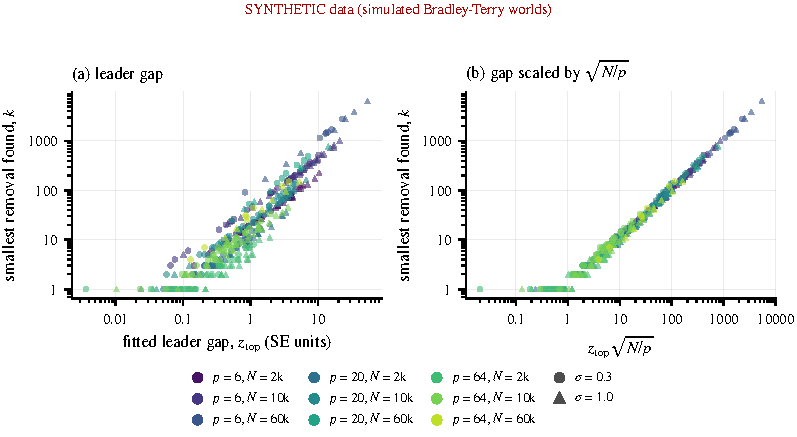
\includegraphics[width=\linewidth]{figA1_synthetic.pdf}\caption{\textbf{Synthetic} Bradley--Terry worlds (not real leaderboards): smallest verified top-1 removal budget (a) against the fitted leader gap $z_{\rm top}$, for several $N$, $p$ and score spreads $\sigma$, and (b) against $z_{\rm top}\sqrt{N/p}$, where the points collapse onto one line (the regression in \texttt{results/summary\_synthetic\_regression.csv}).}\label{fig:synth}\end{figure}

\section{Reproducibility}\label{app:repro}
\paragraph{Reproduction.} Raw data are kept outside the code repository; \texttt{code/00\_fetch\_data.sh} downloads and checks the pinned snapshots:
Arena-55k (Hugging Face \texttt{lmarena-ai/arena-human-preference-55k}, commit \texttt{18c29834}; \texttt{train.csv} sha256 \texttt{0692154a\dots f5be2}),
MT-Bench human and GPT-4 judgments (\texttt{lmsys/mt\_bench\_human\_judgments}, commit \texttt{f7d2896d}; human parquet sha256 \texttt{4877bc46\dots 5769}),
NBA (\texttt{fivethirtyeight/data}, \texttt{nba-elo/nbaallelo.csv}, commit \texttt{4c1ff5e3}; sha256 \texttt{d46ed354\dots 16bc}).
Licences: Arena-55k apache-2.0; MT-Bench judgments cc-by-4.0; NBA data CC-BY-4.0. All experiments ran on CPU (2 cores, shared); the longest single scripts (Arena and NBA attack bootstraps, common-size controls, synthetic calibration) took 10--20 minutes. Software: Python 3.11.2, numpy 2.4.6, scipy 1.17.1, pandas 3.0.6 (\texttt{results/ENV.txt}). Seeds (fixed in the scripts): attack bootstrap resample $r$ uses seed $1000+r$; benign Monte-Carlo 2024; subsample curves 5; MT-Bench contrast 3; common-size controls 77 and Arena controls 78; synthetic worlds 9; equal-size random baselines 11; bootstrap intervals of summary medians 6. The reproduction guide \texttt{REPRODUCE.md} lists environment versions, seeds, commands, run times, and the script that generates each table and figure.
% C5 sensitivity, synthetic calibration (labelled synthetic), reproducibility pointers.

\section*{NeurIPS Paper Checklist}



\begin{enumerate}

\item {\bf Claims}
    \item[] Question: Do the main claims made in the abstract and introduction accurately reflect the paper's contributions and scope?
    \item[] Answer: \answerYes{} % Replace by \answerYes{}, \answerNo{}, or \answerNA{}.
    \item[] Justification: The abstract and introduction state the measured budgets, the comparison with noise, the scale argument and the scope (upper bounds, snapshots, confounded designs); see Sections~\ref{sec:intro}, \ref{sec:results}.
    \item[] Guidelines:
    \begin{itemize}
        \item The answer \answerNA{} means that the abstract and introduction do not include the claims made in the paper.
        \item The abstract and/or introduction should clearly state the claims made, including the contributions made in the paper and important assumptions and limitations. A \answerNo{} or \answerNA{} answer to this question will not be perceived well by the reviewers. 
        \item The claims made should match theoretical and experimental results, and reflect how much the results can be expected to generalize to other settings. 
        \item It is fine to include aspirational goals as motivation as long as it is clear that these goals are not attained by the paper. 
    \end{itemize}

\item {\bf Limitations}
    \item[] Question: Does the paper discuss the limitations of the work performed by the authors?
    \item[] Answer: \answerYes{} % Replace by \answerYes{}, \answerNo{}, or \answerNA{}.
    \item[] Justification: Section~\ref{sec:discussion} lists limitations: upper-bound budgets, optimistic bootstrap intervals, few attack resamples, single BT specification, idealised perturbations, design confounding.
    \item[] Guidelines:
    \begin{itemize}
        \item The answer \answerNA{} means that the paper has no limitation while the answer \answerNo{} means that the paper has limitations, but those are not discussed in the paper. 
        \item The authors are encouraged to create a separate ``Limitations'' section in their paper.
        \item The paper should point out any strong assumptions and how robust the results are to violations of these assumptions (e.g., independence assumptions, noiseless settings, model well-specification, asymptotic approximations only holding locally). The authors should reflect on how these assumptions might be violated in practice and what the implications would be.
        \item The authors should reflect on the scope of the claims made, e.g., if the approach was only tested on a few datasets or with a few runs. In general, empirical results often depend on implicit assumptions, which should be articulated.
        \item The authors should reflect on the factors that influence the performance of the approach. For example, a facial recognition algorithm may perform poorly when image resolution is low or images are taken in low lighting. Or a speech-to-text system might not be used reliably to provide closed captions for online lectures because it fails to handle technical jargon.
        \item The authors should discuss the computational efficiency of the proposed algorithms and how they scale with dataset size.
        \item If applicable, the authors should discuss possible limitations of their approach to address problems of privacy and fairness.
        \item While the authors might fear that complete honesty about limitations might be used by reviewers as grounds for rejection, a worse outcome might be that reviewers discover limitations that aren't acknowledged in the paper. The authors should use their best judgment and recognize that individual actions in favor of transparency play an important role in developing norms that preserve the integrity of the community. Reviewers will be specifically instructed to not penalize honesty concerning limitations.
    \end{itemize}

\item {\bf Theory assumptions and proofs}
    \item[] Question: For each theoretical result, does the paper provide the full set of assumptions and a complete (and correct) proof?
    \item[] Answer: \answerNA{} % Replace by \answerYes{}, \answerNo{}, or \answerNA{}.
    \item[] Justification: The paper has no theorems; the scaling law is estimated empirically on labelled synthetic data.
    \item[] Guidelines:
    \begin{itemize}
        \item The answer \answerNA{} means that the paper does not include theoretical results. 
        \item All the theorems, formulas, and proofs in the paper should be numbered and cross-referenced.
        \item All assumptions should be clearly stated or referenced in the statement of any theorems.
        \item The proofs can either appear in the main paper or the supplemental material, but if they appear in the supplemental material, the authors are encouraged to provide a short proof sketch to provide intuition. 
        \item Inversely, any informal proof provided in the core of the paper should be complemented by formal proofs provided in appendix or supplemental material.
        \item Theorems and Lemmas that the proof relies upon should be properly referenced. 
    \end{itemize}

    \item {\bf Experimental result reproducibility}
    \item[] Question: Does the paper fully disclose all the information needed to reproduce the main experimental results of the paper to the extent that it affects the main claims and/or conclusions of the paper (regardless of whether the code and data are provided or not)?
    \item[] Answer: \answerYes{} % Replace by \answerYes{}, \answerNo{}, or \answerNA{}.
    \item[] Justification: Sections~\ref{sec:method}--\ref{sec:setup}, the appendix and \texttt{REPRODUCE.md} give the model, ridge, tie rules, targets, perturbations, search, datasets (versions and checksums) and seeds.
    \item[] Guidelines:
    \begin{itemize}
        \item The answer \answerNA{} means that the paper does not include experiments.
        \item If the paper includes experiments, a \answerNo{} answer to this question will not be perceived well by the reviewers: Making the paper reproducible is important, regardless of whether the code and data are provided or not.
        \item If the contribution is a dataset and\slash or model, the authors should describe the steps taken to make their results reproducible or verifiable. 
        \item Depending on the contribution, reproducibility can be accomplished in various ways. For example, if the contribution is a novel architecture, describing the architecture fully might suffice, or if the contribution is a specific model and empirical evaluation, it may be necessary to either make it possible for others to replicate the model with the same dataset, or provide access to the model. In general. releasing code and data is often one good way to accomplish this, but reproducibility can also be provided via detailed instructions for how to replicate the results, access to a hosted model (e.g., in the case of a large language model), releasing of a model checkpoint, or other means that are appropriate to the research performed.
        \item While NeurIPS does not require releasing code, the conference does require all submissions to provide some reasonable avenue for reproducibility, which may depend on the nature of the contribution. For example
        \begin{enumerate}
            \item If the contribution is primarily a new algorithm, the paper should make it clear how to reproduce that algorithm.
            \item If the contribution is primarily a new model architecture, the paper should describe the architecture clearly and fully.
            \item If the contribution is a new model (e.g., a large language model), then there should either be a way to access this model for reproducing the results or a way to reproduce the model (e.g., with an open-source dataset or instructions for how to construct the dataset).
            \item We recognize that reproducibility may be tricky in some cases, in which case authors are welcome to describe the particular way they provide for reproducibility. In the case of closed-source models, it may be that access to the model is limited in some way (e.g., to registered users), but it should be possible for other researchers to have some path to reproducing or verifying the results.
        \end{enumerate}
    \end{itemize}


\item {\bf Open access to data and code}
    \item[] Question: Does the paper provide open access to the data and code, with sufficient instructions to faithfully reproduce the main experimental results, as described in supplemental material?
    \item[] Answer: \answerYes{} % Replace by \answerYes{}, \answerNo{}, or \answerNA{}.
    \item[] Justification: Code, result files and \texttt{REPRODUCE.md} (commands, seeds, run times, script for each table and figure) accompany the submission; the datasets are public and fetched by \texttt{code/00\_fetch\_data.sh}.
    \item[] Guidelines:
    \begin{itemize}
        \item The answer \answerNA{} means that paper does not include experiments requiring code.
        \item Please see the NeurIPS code and data submission guidelines (\url{https://neurips.cc/public/guides/CodeSubmissionPolicy}) for more details.
        \item While we encourage the release of code and data, we understand that this might not be possible, so \answerNo{} is an acceptable answer. Papers cannot be rejected simply for not including code, unless this is central to the contribution (e.g., for a new open-source benchmark).
        \item The instructions should contain the exact command and environment needed to run to reproduce the results. See the NeurIPS code and data submission guidelines (\url{https://neurips.cc/public/guides/CodeSubmissionPolicy}) for more details.
        \item The authors should provide instructions on data access and preparation, including how to access the raw data, preprocessed data, intermediate data, and generated data, etc.
        \item The authors should provide scripts to reproduce all experimental results for the new proposed method and baselines. If only a subset of experiments are reproducible, they should state which ones are omitted from the script and why.
        \item At submission time, to preserve anonymity, the authors should release anonymized versions (if applicable).
        \item Providing as much information as possible in supplemental material (appended to the paper) is recommended, but including URLs to data and code is permitted.
    \end{itemize}


\item {\bf Experimental setting/details}
    \item[] Question: Does the paper specify all the training and test details (e.g., data splits, hyperparameters, how they were chosen, type of optimizer) necessary to understand the results?
    \item[] Answer: \answerNA{} % Replace by \answerYes{}, \answerNo{}, or \answerNA{}.
    \item[] Justification: There is no training or test split: we fit Bradley--Terry models by Newton's method on the full comparison data; the ridge value is fixed in Section~\ref{sec:method} and varied in Appendix Table~\ref{tab:sens}.
    \item[] Guidelines:
    \begin{itemize}
        \item The answer \answerNA{} means that the paper does not include experiments.
        \item The experimental setting should be presented in the core of the paper to a level of detail that is necessary to appreciate the results and make sense of them.
        \item The full details can be provided either with the code, in appendix, or as supplemental material.
    \end{itemize}

\item {\bf Experiment statistical significance}
    \item[] Question: Does the paper report error bars suitably and correctly defined or other appropriate information about the statistical significance of the experiments?
    \item[] Answer: \answerYes{} % Replace by \answerYes{}, \answerNo{}, or \answerNA{}.
    \item[] Justification: Bootstrap and Monte-Carlo intervals are reported with the number of resamples; Arena and NBA attack bootstraps use only 20 resamples (6 for $\tau$), stated in Table~\ref{tab:summary} and Section~\ref{sec:discussion}; no significance tests are claimed.
    \item[] Guidelines:
    \begin{itemize}
        \item The answer \answerNA{} means that the paper does not include experiments.
        \item The authors should answer \answerYes{} if the results are accompanied by error bars, confidence intervals, or statistical significance tests, at least for the experiments that support the main claims of the paper.
        \item The factors of variability that the error bars are capturing should be clearly stated (for example, train/test split, initialization, random drawing of some parameter, or overall run with given experimental conditions).
        \item The method for calculating the error bars should be explained (closed form formula, call to a library function, bootstrap, etc.)
        \item The assumptions made should be given (e.g., Normally distributed errors).
        \item It should be clear whether the error bar is the standard deviation or the standard error of the mean.
        \item It is OK to report 1-sigma error bars, but one should state it. The authors should preferably report a 2-sigma error bar than state that they have a 96\% CI, if the hypothesis of Normality of errors is not verified.
        \item For asymmetric distributions, the authors should be careful not to show in tables or figures symmetric error bars that would yield results that are out of range (e.g., negative error rates).
        \item If error bars are reported in tables or plots, the authors should explain in the text how they were calculated and reference the corresponding figures or tables in the text.
    \end{itemize}

\item {\bf Experiments compute resources}
    \item[] Question: For each experiment, does the paper provide sufficient information on the computer resources (type of compute workers, memory, time of execution) needed to reproduce the experiments?
    \item[] Answer: \answerYes{} % Replace by \answerYes{}, \answerNo{}, or \answerNA{}.
    \item[] Justification: CPU only (2 cores); Appendix~\ref{app:repro} and \texttt{REPRODUCE.md} give the run time of every script (minutes up to about 20 minutes each on shared hardware).
    \item[] Guidelines:
    \begin{itemize}
        \item The answer \answerNA{} means that the paper does not include experiments.
        \item The paper should indicate the type of compute workers CPU or GPU, internal cluster, or cloud provider, including relevant memory and storage.
        \item The paper should provide the amount of compute required for each of the individual experimental runs as well as estimate the total compute. 
        \item The paper should disclose whether the full research project required more compute than the experiments reported in the paper (e.g., preliminary or failed experiments that didn't make it into the paper). 
    \end{itemize}
    
\item {\bf Code of ethics}
    \item[] Question: Does the research conducted in the paper conform, in every respect, with the NeurIPS Code of Ethics \url{https://neurips.cc/public/EthicsGuidelines}?
    \item[] Answer: \answerYes{} % Replace by \answerYes{}, \answerNo{}, or \answerNA{}.
    \item[] Justification: The study uses public datasets only, no human subjects and no private data; we see no violation of the Code of Ethics.
    \item[] Guidelines:
    \begin{itemize}
        \item The answer \answerNA{} means that the authors have not reviewed the NeurIPS Code of Ethics.
        \item If the authors answer \answerNo, they should explain the special circumstances that require a deviation from the Code of Ethics.
        \item The authors should make sure to preserve anonymity (e.g., if there is a special consideration due to laws or regulations in their jurisdiction).
    \end{itemize}


\item {\bf Broader impacts}
    \item[] Question: Does the paper discuss both potential positive societal impacts and negative societal impacts of the work performed?
    \item[] Answer: \answerYes{} % Replace by \answerYes{}, \answerNo{}, or \answerNA{}.
    \item[] Justification: Section~\ref{sec:discussion} discusses the auditing benefit and the risk that the method is a recipe for manipulating leaderboards.
    \item[] Guidelines:
    \begin{itemize}
        \item The answer \answerNA{} means that there is no societal impact of the work performed.
        \item If the authors answer \answerNA{} or \answerNo, they should explain why their work has no societal impact or why the paper does not address societal impact.
        \item Examples of negative societal impacts include potential malicious or unintended uses (e.g., disinformation, generating fake profiles, surveillance), fairness considerations (e.g., deployment of technologies that could make decisions that unfairly impact specific groups), privacy considerations, and security considerations.
        \item The conference expects that many papers will be foundational research and not tied to particular applications, let alone deployments. However, if there is a direct path to any negative applications, the authors should point it out. For example, it is legitimate to point out that an improvement in the quality of generative models could be used to generate Deepfakes for disinformation. On the other hand, it is not needed to point out that a generic algorithm for optimizing neural networks could enable people to train models that generate Deepfakes faster.
        \item The authors should consider possible harms that could arise when the technology is being used as intended and functioning correctly, harms that could arise when the technology is being used as intended but gives incorrect results, and harms following from (intentional or unintentional) misuse of the technology.
        \item If there are negative societal impacts, the authors could also discuss possible mitigation strategies (e.g., gated release of models, providing defenses in addition to attacks, mechanisms for monitoring misuse, mechanisms to monitor how a system learns from feedback over time, improving the efficiency and accessibility of ML).
    \end{itemize}
    
\item {\bf Safeguards}
    \item[] Question: Does the paper describe safeguards that have been put in place for responsible release of data or models that have a high risk for misuse (e.g., pre-trained language models, image generators, or scraped datasets)?
    \item[] Answer: \answerNA{} % Replace by \answerYes{}, \answerNo{}, or \answerNA{}.
    \item[] Justification: We release no model or new dataset; only analysis code and derived result tables of public data.
    \item[] Guidelines:
    \begin{itemize}
        \item The answer \answerNA{} means that the paper poses no such risks.
        \item Released models that have a high risk for misuse or dual-use should be released with necessary safeguards to allow for controlled use of the model, for example by requiring that users adhere to usage guidelines or restrictions to access the model or implementing safety filters. 
        \item Datasets that have been scraped from the Internet could pose safety risks. The authors should describe how they avoided releasing unsafe images.
        \item We recognize that providing effective safeguards is challenging, and many papers do not require this, but we encourage authors to take this into account and make a best faith effort.
    \end{itemize}

\item {\bf Licenses for existing assets}
    \item[] Question: Are the creators or original owners of assets (e.g., code, data, models), used in the paper, properly credited and are the license and terms of use explicitly mentioned and properly respected?
    \item[] Answer: \answerYes{} % Replace by \answerYes{}, \answerNo{}, or \answerNA{}.
    \item[] Justification: Datasets are credited and their licences stated (apache-2.0, cc-by-4.0, CC-BY-4.0; Appendix~\ref{app:repro}); we did not use the data whose licence is undeclared or restricted.
    \item[] Guidelines:
    \begin{itemize}
        \item The answer \answerNA{} means that the paper does not use existing assets.
        \item The authors should cite the original paper that produced the code package or dataset.
        \item The authors should state which version of the asset is used and, if possible, include a URL.
        \item The name of the license (e.g., CC-BY 4.0) should be included for each asset.
        \item For scraped data from a particular source (e.g., website), the copyright and terms of service of that source should be provided.
        \item If assets are released, the license, copyright information, and terms of use in the package should be provided. For popular datasets, \url{paperswithcode.com/datasets} has curated licenses for some datasets. Their licensing guide can help determine the license of a dataset.
        \item For existing datasets that are re-packaged, both the original license and the license of the derived asset (if it has changed) should be provided.
        \item If this information is not available online, the authors are encouraged to reach out to the asset's creators.
    \end{itemize}

\item {\bf New assets}
    \item[] Question: Are new assets introduced in the paper well documented and is the documentation provided alongside the assets?
    \item[] Answer: \answerYes{} % Replace by \answerYes{}, \answerNo{}, or \answerNA{}.
    \item[] Justification: The released code and result files are documented in \texttt{REPRODUCE.md} and \texttt{results/SCHEMA.md}.
    \item[] Guidelines:
    \begin{itemize}
        \item The answer \answerNA{} means that the paper does not release new assets.
        \item Researchers should communicate the details of the dataset\slash code\slash model as part of their submissions via structured templates. This includes details about training, license, limitations, etc. 
        \item The paper should discuss whether and how consent was obtained from people whose asset is used.
        \item At submission time, remember to anonymize your assets (if applicable). You can either create an anonymized URL or include an anonymized zip file.
    \end{itemize}

\item {\bf Crowdsourcing and research with human subjects}
    \item[] Question: For crowdsourcing experiments and research with human subjects, does the paper include the full text of instructions given to participants and screenshots, if applicable, as well as details about compensation (if any)? 
    \item[] Answer: \answerNA{} % Replace by \answerYes{}, \answerNo{}, or \answerNA{}.
    \item[] Justification: We did not run crowdsourcing; we analyse existing public votes.
    \item[] Guidelines:
    \begin{itemize}
        \item The answer \answerNA{} means that the paper does not involve crowdsourcing nor research with human subjects.
        \item Including this information in the supplemental material is fine, but if the main contribution of the paper involves human subjects, then as much detail as possible should be included in the main paper. 
        \item According to the NeurIPS Code of Ethics, workers involved in data collection, curation, or other labor should be paid at least the minimum wage in the country of the data collector. 
    \end{itemize}

\item {\bf Institutional review board (IRB) approvals or equivalent for research with human subjects}
    \item[] Question: Does the paper describe potential risks incurred by study participants, whether such risks were disclosed to the subjects, and whether Institutional Review Board (IRB) approvals (or an equivalent approval/review based on the requirements of your country or institution) were obtained?
    \item[] Answer: \answerNA{} % Replace by \answerYes{}, \answerNo{}, or \answerNA{}.
    \item[] Justification: We conducted no research with human subjects; we analyse existing public data.
    \item[] Guidelines:
    \begin{itemize}
        \item The answer \answerNA{} means that the paper does not involve crowdsourcing nor research with human subjects.
        \item Depending on the country in which research is conducted, IRB approval (or equivalent) may be required for any human subjects research. If you obtained IRB approval, you should clearly state this in the paper. 
        \item We recognize that the procedures for this may vary significantly between institutions and locations, and we expect authors to adhere to the NeurIPS Code of Ethics and the guidelines for their institution. 
        \item For initial submissions, do not include any information that would break anonymity (if applicable), such as the institution conducting the review.
    \end{itemize}

\item {\bf Declaration of LLM usage}
    \item[] Question: Does the paper describe the usage of LLMs if it is an important, original, or non-standard component of the core methods in this research? Note that if the LLM is used only for writing, editing, or formatting purposes and does \emph{not} impact the core methodology, scientific rigor, or originality of the research, declaration is not required.
    %this research? 
    \item[] Answer: \answerYes{} % Replace by \answerYes{}, \answerNo{}, or \answerNA{}.
    \item[] Justification: Section~\ref{sec:setup} discloses that an LLM (Claude via Claude Code) assisted with literature reading, code, analysis and writing; all reported numbers come from the shipped code.
    \item[] Guidelines:
    \begin{itemize}
        \item The answer \answerNA{} means that the core method development in this research does not involve LLMs as any important, original, or non-standard components.
        \item Please refer to our LLM policy in the NeurIPS handbook for what should or should not be described.
    \end{itemize}

\end{enumerate}
\end{document}
